\chapter{Comparison of modern Java Script Frameworks}

\section{Open Questions}

just for me....
\begin{itemize}
	\item Security issues of templating systems (especially XSS)
	\item differences of dom based vs string based templates
	\item is there a difference between templates and data binding?
\end{itemize}
 
\section{Overview}

There is a huge and steadily increasing amount of new JS MV* frameworks. (prove this with literature, show both pictures of ToDoMVC App). A good overview over existing projects is provided by the Todo MVC App (Quelle TodoMVC)
The Todo MVC app was created with the intention to help developers selecting a JavaScript framework by providing implementations of the very simple and ever same 
ToDo App, which allows to define a set of tasks that need to be done. The application allows to add/delete/edit todo tasks and to mark/unmark tasks as done/undone. The TodoMVC app gives also a good evidence of the rapid increase of existing JavaScript MVC frameworks. Figure XX shows a screenshot of the ToDoMVC taken at two different dates with a period of year.

\begin{figure}
	\centering	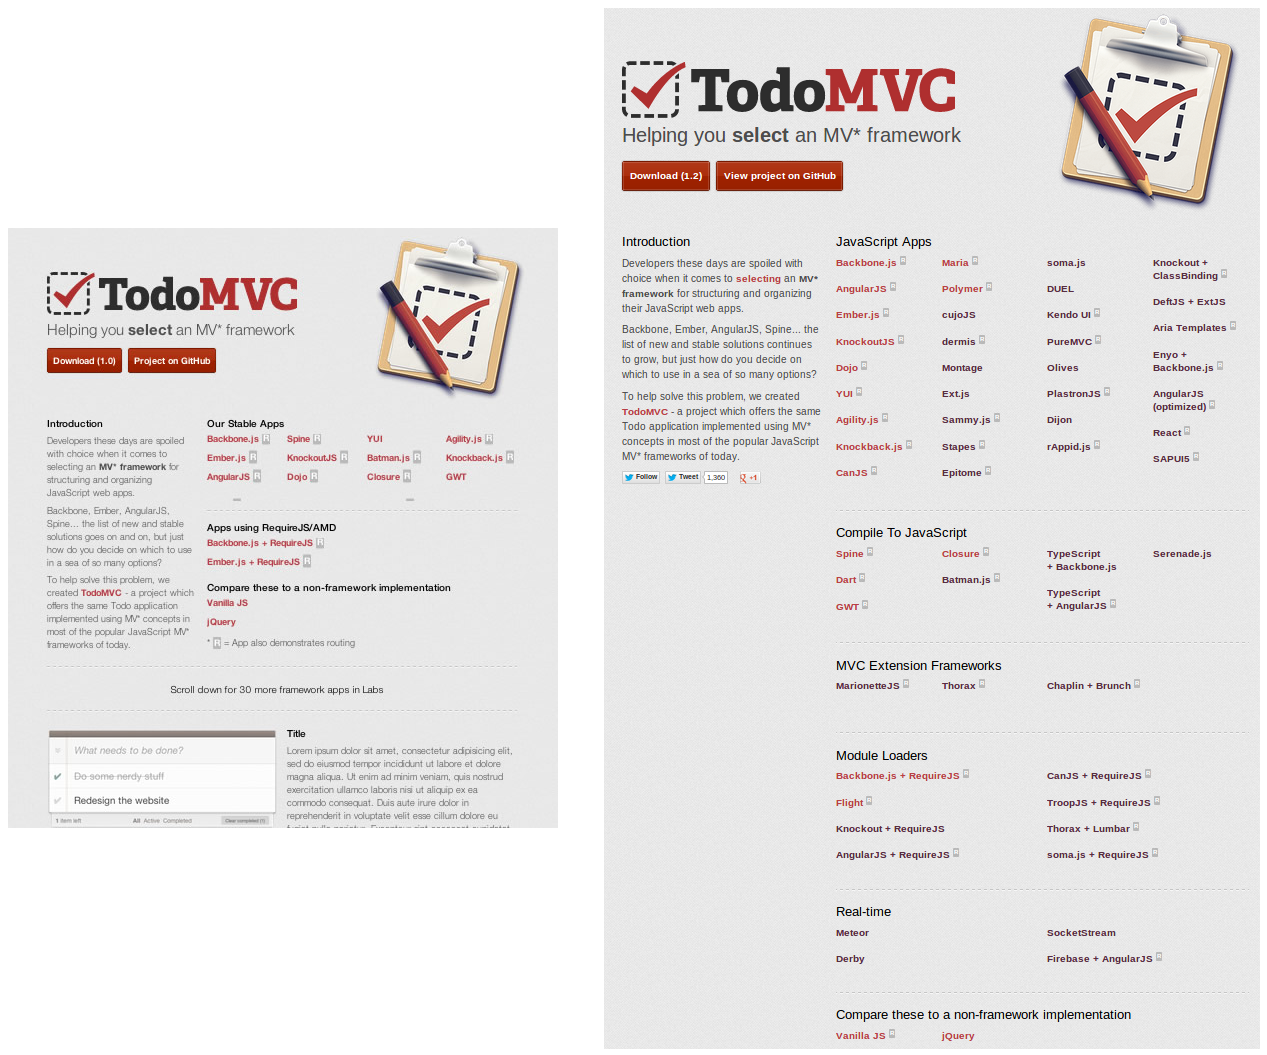
\includegraphics[width=1.0\textwidth]{./img/todo_mvc_app_comparison.png}
	\caption{Screenshot TodoMVC app left:July 2012, right: August 2013~}
	\label{fig:todoMvcComp}
\end{figure}
    

The large amount of different frameworks makes it impossible to examine them all in very detail. Therefore a two step approach to filter the best suiting candidate is applied. In a first step a very rough comparison of the frameworks is made to filter out the most inappropriate frameworks. The remaining frameworks are then in a second step examinied in more detail. Furthermore a simple application is implemented with the different frameworks to get a better understandig of them. The implemented application is a simple cids renderer for an example vermessungriss bean taken from wunda. This example was choosen since such renderer are one part that will be implemented in future.    

The following list shows relevant JS MV* frameworks taken from the ToDoMVC app. The list only contains frameworks wich are available in a stable release (at least 1.0.0), availabe as open source. Furthermore a combinations of different apis are also excluded 

\begin{itemize}
	\item Dojo
	\item YUI
	\item CanJS
	\item soma.js
	\item Maria
	\item Backbone JS
	\item AngularJS
	\item Ember JS
	\item Knockout JS
\end{itemize}

Dojo as well as YUI (Yahoo! User Interface) arent MV* frameworks in the proper meaning of an MV* Framework. They are, like JQuery, DOM/Ajax wrapping libraries. Both has several addiational features like ui-elements, effects and animations. Both doesn't implement the MVC pattern and dont provide the user with built in features like data binding, templating or routing and are therefore not taken into further considerations.


CanJS, Soma.js and Maria are very new MVC Frameworks all providing a different set of the basic features like data-binding, templating and routing. According to [http://de.slideshare.net/moschel/canjs-the-best-of-both-worlds] CanJS combines the best features of lightweight frameworks like BackboneJS, which are easy to learn have and small size, as well as of heavy frameworks like ember js which offer a lot of good features like live binding,computed properties and memory safety. CanJS can use EJS or Mustache as templating engines which are both string based temoplating engines. In one sentence CanJS can be  characterized through its high performance, its memory leak prevention and the fact that it can be used with a lot of different DOM libraries. Although soma.js can be used as a MVC framework the basic idea behind soma.js is a more general approach. "soma.js  provides tools to create a loosely-coupled architecture broken down into smaller pieces." [soma website] In order to do so, it implements a large set of different design patterns, like dependency injection, observer pattern or mediator pattern. Soma.js implements its own template engine based on soma.js.
The authors of Maria emphasize that this framework implements the "real" MVC pattern. Maria is a very leightweight framework which means that there is no built in support for templates and data binding which mean that it is necessary to write a lot of boilerplate code on your own.


Generally speaking, the problem with these very young frameworks is, that these projects are not so well documented and there is only a small community which makes it very difficult to find information or help when problems occur. This disqualifies these frameworks as possible candidate.


One of the more matured and proven frameworks is Backbone JS. A lot of really large and impressive projects are built with backbone.js such as  LinkedIn, AirBnB, Trello, or FourSquare. Hence its maturity, it is well documented and there is a large and active community which makes it easy to find help. Backbone JS is a very flexible library since it consists of different modules concerning single aspects of web application creation such as controllers, routers and so on. Thus it defines a structure for the application. Hence it has a flexible and minimalistic approach it is necessary to write a lot of boilerplate code. Backbone JS is not able to reflect changed model data to the view and vice verca (no two way data binding). To achieve this it is necessary to hook on different events that are fired when the view or model changes and then updating the information manually. 


- Backbone is build to work with rest apis as backend. 


- Uses underscore as templating systems


- Why cant we use Backbone????


\section{Comparison of AngularJS, EmberJS and KnockoutJS}


\textbf{Angular JS}  

AngularJS is developed by Google and has become one of the more popular Frameworks. Angular JS follows a slightly different apporach compared to the other frameworks. This approach is best described by the angular developers itself: Angular is what HTML would have been had it been designed for applications (angular documentation). One aspect that shows the difference of angular are the so called directives. Directives allow the user to extend the native html with new and application dependent functionality.  This is done by introducing new html tags and some javascript code that defines the semantics/behaviour of this tag as well as a way how to convert the new introduced tag and the current model state into plain old html (example?!). Using directives extensively, "HTML can be turned into a declarative domain specific language (DSL)" (Zitat angular doc)
  
The second aspect Angular differs from the other frameworks is the templating system. (angular docu says that the template system is DOM based ?)   

Besides these features Angular JS also provides two way data binding, filters, routing and dependency injection. 
All these components and features make it easy to write single page web applications without writing any sort of boilerplate code, assumed that you are familiar with the architecture and concepts of Angular JS. (this is one the disadvantages, takes much time to get familiar with angular)  

- is the one with the most community activity (github forks, stars, watches) 
	

\textbf{Ember JS}

Ember JS is one of the younger frameworks out there, mainly created by Yehuda Katz and Tom Dale and introduced in December 2011 (see link yehuda katz blog). in this short time Ember JS could make really impressive progress and has gained a lot of attraction (github forks, stars, watches). It comprises all necessary parts for building web applications including two way data binding with templates, a routing mechanism and provides a way to connect the application to a REST api.
Ember is a very stringent and opinionated framework and is built upon concepts such as DRY (dont repeat yourself) and CoC (Convention over Configuration). Especially the usage of naming conventions allows it to write applications with a dramatically less code, in fact Ember.js abstract boilerplate code. The disadvantage of this is that it is more sophisticated to get started with Ember.js because you have to get into the ember zen (TODO rewrite this). Furthermore this makes Ember one of the largest framewworks (56kb)
It uses Handlebars as its templating engine, which is a very popular string based templating enginge. Ember.js also provides a way to connect your application to RESTful WebServices with an additional project Ember-Data. As well as Ember.js Ember-Data makes highly use of the Convention over Configuration principle which means that Ember-Data expects the data provided by a REST-Service in a special format. The Ember team substantiate : "[...]we don't think most web developers should have to write any custom XHR code for loading data. Strong conventions on the client and strong conventions on the server should allow them to communicate automatically." (Ember website stabilizing ember data). Besides Ember-Data it is also possible to use any other server connection implementation.         



\textbf{Knockout JS}  Knockout JS is a more leightweight library, which only implents the MVVM pattern for HTML which brings two way data binding and a seperation of gui logic/state from the gui itself. The two way data binding is implemented by using special Java Script Objects (Knockout Observables) provided by Knockout, which can notify the view/model about changes.(Bild Knockout MVVM from heise Developer) Knockout JS doesn't support you by attaching a server side backend. Furthermore it is not able to route between different pages of your application. Knockout JS very reduced feature set can be both, a blessing and a curse and it depends on the needs to decide what of these two things prevails. Knockout JS is a very easy to learn library hence there are only a few concepts to learn. Another benefit of Knockout JS is, that it has a widely spreaded browser support also for older browser versions. It is a very flexible framework hence there are  no regulations for defining the structure and architecture of your application. The missing features of Knockout JS like routing can be compensated with one of the other dozen available third party libraries for this feature. Unfortunately, without these additional dependencies Knockout JS is rather less suited for building web applications in fact that it forces you to implement too many things manually. And the additional amount of dependencies could lead to inconsitency problems, increases the error likelyhood and the maintenance efforts and make the development event harder. (vgl artice heise online)     

\begin{landscape}
	\begin{longtable}{| p{5cm} | p{5cm} | p{5cm} | p{5cm} |}
	\hline
		& Angular JS				
		& Ember JS	
		& Knockout JS \\ \hline
	2-way binding	 		
		& \checkmark
		& \checkmark
		& \checkmark  \\ \hline
	normal / computed properties	
		& \checkmark / change detection
		& \checkmark / \checkmark
		& \checkmark / \checkmark\\ \hline
	Testing				
		& very easy, end-to-end test, build in tools for unit tests, 
		  end to end test (gui tests), tools for testing app in realtime with different browsers 
		& extra packages ember-testing,qUnit 
		&  unit tests \\ \hline
	Routing				
		& \checkmark 
		& \checkmark	
		& -		\\ \hline
	Multiple / Composite Views	
		& \checkmark / \checkmark
		& \checkmark / \checkmark 
		& -		\\ \hline
	Backend connection		
		& optional (ajax wrapper)	
		& optional (ember-data)	
		& -	\\ \hline
	Dependency injection
		& \checkmark
		& -
		& -\\ \hline
	Templating system
		& Dom based 
		& String based (handlebars)
		& Dom based\\ \hline
	Documentation
		& very good
		& good
		& good\\ \hline
	API stability / maturity
		& Initial release 2009, curr 1.0.7
		& Inital release 2011, curr ember 1.0.0-rc6.1
		& First version 2010, current 2.3.0\\ \hline
	community (github watch/star/fork
		& 1450/13061/3147
		& 672/7752/1568
		& 349/4074/657\\ \hline
	Security
		&
		&
		& \\ \hline
	Perfomance
		&
		&
		& \\ \hline
	Flexibile vs opinonated
		& flexible
		& stringent \& opinionated
		& very flexible\\ \hline
	size
		& 80kb
		& 56kb + JQuery + Handlebars
		& 15kb\\ \hline	
	FrameWork / Library
		& Something in between
		& Framework
		& Library\\ \hline
	Allows integration of ui elements
		& \checkmark use directives
		& \checkmark use Ember views
		& \checkmark use custom bindings \\ \hline
	\end{longtable}
\end{landscape}


\section{Discussion}

- Ember JS has very good parts which allow to build webapps with little code.  is very strict and opinionated.  
